\documentclass[11pt]{article}
\usepackage{amsmath}
\usepackage{caption}

\usepackage{algorithmicx}
\usepackage{algpseudocode}
\usepackage{algorithm}

\usepackage{graphicx}

\title{Exercisesheet No.1}
\author{Alexander Diete \and Magnus M\"uller \and Martin Pfannem\"uller}

\begin{document}
\maketitle
\section*{Exercise 1}
The agent is rational because it ends in a finite state. At most the agent uses three operations to behave correctly. To prove the rationality in this simple case it is possible to enumerate all possible outcomes of the world:

\begin{itemize}
  \item Case: both squares are dirty
  \begin{itemize}
    \item Robot starts left: \textit{clean, right, clean}
    \item Robot starts right: \textit{clean, left, clean} 
  \end{itemize}
  \item Case: left square is dirty
  \begin{itemize}
    \item Robot starts left: \textit{clean, right}
    \item Robot starts right: \textit{left, clean} 
  \end{itemize}
  \item Case: right square is dirty
  \begin{itemize}
    \item Robot starts left: \textit{right, clean}
    \item Robot starts right: \textit{clean, left} 
  \end{itemize}
  \item Case: no square is dirty
  \begin{itemize}
    \item Robot starts left: \textit{right}
    \item Robot starts right: \textit{left} 
  \end{itemize}
\end{itemize}

\noindent
By definition a rational agent is supposed to maximize its performance measure. It is easy to see that the agent always acts correctly. Thus, it maximizes it's performance and there is no agent that can do better. Therefore we can sufficiently say the agent is rational. 

\newpage

\section*{Exercise 2}
\subsection*{a)}
No it is not a rational agent as it doesn't stop once every square is cleaned. Instead it keeps moving, thus earning penalty points by every move it takes.

\subsection*{b)}
The cleaner stops once it visited all squares as it has a map of the squares. As there is no cleaner that performs better under this environment it is a rational cleaner. (The only assumption is that there exists no cleaner that knows the distribution of the dirty squares a priori)
 
\subsection*{c)}
the agent knows the state of the environment then the agent knows exactly what to do next. For the agent there is a mapping of actions to each of the eight states. Thus this simple reflex agent is rational in this environment.
As the model-based agent/ reflex agent with state is a more sophisticated agent than the simple reflex agent it is rational as well.


\newpage

\section*{Exercise 3}
\subsection*{a)}
No, the simple reflex agent will be trapped in a corner forever once it hits a wall.

\subsection*{b)}
Yes, the randomized agent can outperform the simple reflex agent.
The agent function could look like this: \\
\textbf{function} randomizedAgentFunction (percept) \textbf{returns} an action
\begin{algorithmic}
\If {$dirty$}
    \State return $clean$
\Else
    \State return $randomDirection$
\EndIf
\end{algorithmic}
Eventually the agent using this function will clean all dirty squares.

\subsection*{c)}

\begin{figure}[ht]
	\centering
  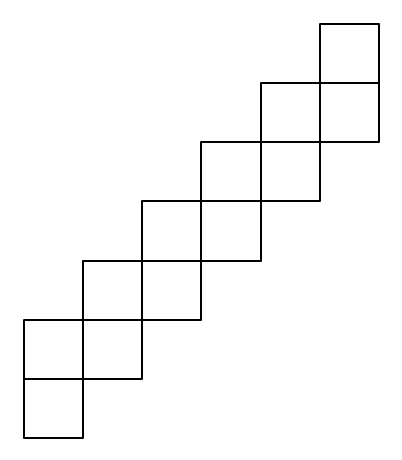
\includegraphics[width=0.3\textwidth]{environment}
	\caption{Hard environment}
	\label{fig:environment}
\end{figure}

\noindent The randomized agent will perform poor in environments with many corners and small paths or in general environments with many edges where you can not go.
\newpage
\section*{Exercise 4}
\subsection*{a)}
\begin{quotation}\noindent
\textit{There exists task environment in which no pure reflex agent can behave rationally.}
\end{quotation}
\noindent
This statement is \textbf{true}. We consider for instance the vacuum-cleaner example with an environment that is not fully observable and also consists of obstacles and other traps. A reflex based agent is not able to act rationally wihtout having some sort of state.

\subsection*{b)}
\begin{quotation}\noindent
\textit{There exists task environment in which every agent is rational.}
\end{quotation}
\noindent
This statement is \textbf{false}. For every environment an agent is able to behave the exact opposite of what it is supposed to do.

\subsection*{c)}
\begin{quotation}\noindent
\textit{The input to an agent function is the same as the input to the agent problem.}
\end{quotation}
\noindent
This statement is \textbf{false}. The agent function may be working on a partially solved problem and may be called multiple times in the program. The input of the agent problem on the other hand is the starting point of the agent.

\subsection*{d)}
\begin{quotation}\noindent
\textit{There can be more than one agent program that implements a given agent function.}
\end{quotation}
\noindent
This statement is \textbf{true}. The agent function is a formal description mapping any percept sequence to an action. There can be multiple different implementations of this formal description.

\subsection*{e)}
\begin{quotation}\noindent
\textit{An agent that senses only partial information about the state cannot be perfectly rational.}
\end{quotation}
\noindent
This statement is \textbf{false}. Missing (sensorial) information can e.g. be compensated by saving an internal state. This means, although an agent cannot sense every information needed, it can act rationally.

\newpage

\section*{Exercise 5}
We cann simply solve this exercise by using truth tables and counting the positive Results. It is important to note, that if a Variable is not mentioned in the preposition, its value is not important for the model and can be either \textbf{true} or \textbf{false}.

\subsection*{a)} 
$(A \wedge B) \vee (B \wedge C)$
\begin{table}[h]
  \begin{tabular}{c|c|c||c}
    A & B & C & Result\\
    \hline
    0 & 0 & 0 & 0 \\
    1 & 0 & 0 & 0 \\
    0 & 1 & 0 & 0 \\
    1 & 1 & 0 & 1 \\
    0 & 0 & 1 & 0 \\
    1 & 0 & 1 & 0 \\
    0 & 1 & 1 & 1 \\
    1 & 1 & 1 & 1
  \end{tabular}
  \caption*{We thus have 3 positive outcomes in the truth-table. As D is not considered in the propositions, its value is not important and can be either true or false. This doubles the result-size to \textbf{6 possible models}.}
\end{table}

\subsection*{b)} 
$A \vee B$
\begin{table}[h]
  \begin{tabular}{c|c||c}
    A & B & Result\\
    \hline
    0 & 0 & 0 \\
    1 & 0 & 1 \\
    0 & 1 & 1 \\
    1 & 1 & 1 
  \end{tabular}
  \caption*{This preposotion also has three positive outcomes but in contrast to \textit{a)} both C and D and not bound in the formula. Therefore any combination of assingment of C and D is valid. This results in $3 \cdot 2^2 = \textbf{12}$ \textbf{possible models}}
\end{table}

\newpage

\subsection*{c)} 
$A \Leftrightarrow  B \Leftrightarrow  C$
\begin{table}[h]
  \begin{tabular}{c|c|c||c}
    A & B & C & Result\\
    \hline
    0 & 0 & 0 & 1 \\
    1 & 0 & 0 & 0 \\
    0 & 1 & 0 & 0 \\
    1 & 1 & 0 & 0 \\
    0 & 0 & 1 & 0 \\
    1 & 0 & 1 & 0 \\
    0 & 1 & 1 & 0 \\
    1 & 1 & 1 & 1
  \end{tabular}
  \caption*{The results are similar to \textit{a)} as D is unbound. This results in $2 \cdot 2 = \textbf{4}$ \textbf{possible models}.}
\end{table}

\subsection*{d)} 
$A \wedge  B \wedge \neg D$
\begin{table}[h]
  \begin{tabular}{c|c|c||c}
    A & B & D & Result\\
    \hline
    0 & 0 & 0 & 0 \\
    1 & 0 & 0 & 0 \\
    0 & 1 & 0 & 0 \\
    1 & 1 & 0 & 1 \\
    0 & 0 & 1 & 0 \\
    1 & 0 & 1 & 0 \\
    0 & 1 & 1 & 0 \\
    1 & 1 & 1 & 0
  \end{tabular}
  \caption*{The results are similar to \textit{a)} or \textit{c)}. But in this case C is unbound. This results in $1 \cdot 2 = \textbf{2}$ \textbf{possible models}.}
\end{table}

\newpage
\section*{Exercise 6}
\subsection*{a)}
If $\alpha$ is valid, then it is true. Therefore true always is a subset of/entails $\alpha$ (see definition).

\subsection*{b)}
If $\alpha$ is false, then false $\models$ false which is obviously true
If $\alpha$ is true, then false $\models$ true which is true as well
Thus the assertion is true.

\subsection*{c)}
\begin{table}[h]
  \begin{tabular}{c|c||c|c}
    $\alpha$ & $\beta$ & $\neg \alpha \vee \beta$ & $\alpha \subseteq \beta$\\
    \hline
    0 & 0 & 1 & 1\\
    0 & 1 & 1 & 1\\
    1 & 0 & 0 & 0\\
    1 & 1 & 1 & 1\\
  \end{tabular}
  \caption*{It follows from the table that the assertion is true.}
\end{table}

\subsection*{d)}
\begin{table}[h]
  \begin{tabular}{c|c||c|c}
    $\alpha$ & $\beta$ & $\alpha \Leftrightarrow \beta$ & $\alpha \equiv \beta$\\
    \hline
    0 & 0 & 1 & 1\\
    0 & 1 & 0 & 0\\
    1 & 0 & 0 & 0\\
    1 & 1 & 1 & 1\\
  \end{tabular}
  \caption*{It follows from the table that the assertion is true.}
\end{table}

\subsection*{e)}
\begin{table}[h]
  \begin{tabular}{c|c||c|c|c}
    $\alpha$ & $\beta$ & $\alpha \wedge \neg \beta$ & $\neg \alpha \vee \beta$ & $\alpha \models \beta$\\
    \hline
    0 & 0 & 0 & 1 & 1\\
    0 & 1 & 0 & 1 & 1\\
    1 & 0 & 1 & 0 & 0\\
    1 & 1 & 0 & 1 & 1\\
  \end{tabular}
  \caption*{It follows from the table that the assertion is true.}
\end{table}
\end{document}

